%!TEX root = ../doc.tex
\chapter{Umsetzung des Prototyps}
\label{sec:umsetzung}

\section{Vorbereitung}
Für die Entwicklung des Prototypen wird Android Studio Version 1.2 von Google verwendet. Android Studio baut auf der freien Version von IntelliJ IDEA auf und verfügt daher über sehr viele nützliche Entwicklerwerkzeuge. Für die Versionskontrolle des Quellecodes wird Git und eine Repository auf Github\footnote{Repository auf Github: \url{https://github.com/roosnic1/wifi_action}} verwendet. Für das Testen der App wird ein Android Mobiltelefon des Types Nexus 5 mit der Android Version 5.1 verwendet. Das Android Projekt wird mit der neusten Android SDK Version entwickelt. Das bedeutet die App funktioniert nur auf Mobiltelefonen mit der Android Verison 5.1 dafür können die neusten Funktionen vom SDK verwendet werden. Die Dokumentation bzw. der Entwicklerbericht wird in Sublime Text 3 mit \LaTeX{} geschrieben.

\section{Entwicklung}
Für die Umsetzung der App werden im wesentlichen Activities, für die Darstellungen und Interaktionen mit dem Benutzer, sowie ein Receiver und ein Service benötigt. Dazu kommen noch Adapters und Modelle mit welchen Daten in einer Datenbank bzw. in eine Datei serialisiert werden können. Die einzelnen Komponenten werden in diesem Kapitel beschrieben und auf wichtige Eigenschaften wird hingewiesen.

\subsection{Activities}
In Android repräsentieren Activities eine Benutzeroberfläche. Für die App wurden 3 Activities verwendet, welche mit ihren Verbindungen in der Abbildung \ref{fig:activities} dargestellt sind.

% MainActivity->ActionActivity: open
% note over ActionActivity: create Action
% ActionActivity->MainActivity: return Action
% MainActivity->Action List: save Action
% MainActivity->LogActivity: open
% note over LogActivity: show Logs
\begin{figure}[ht]
    \centering
    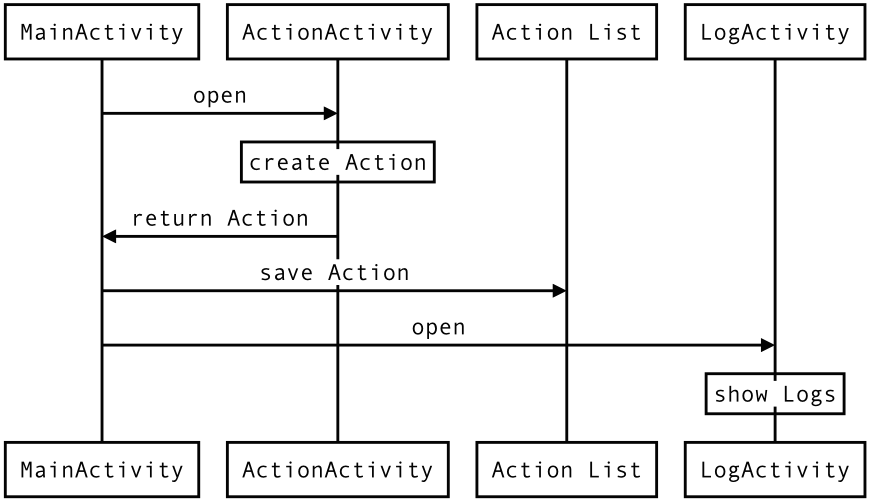
\includegraphics[width=0.7\textwidth]{images/activities.png}
    \caption{Sequenzdiagramm der verwendeten Activities}
    \label{fig:activities}
\end{figure}


\subsubsection{MainActivity}
Die MainActivity ist die Ansicht welche dem Benutzer angezeigt wird wenn der Benutzer die App startet. Wie in der Abbildung \ref{fig:mainactivity} beinhaltet die Activity in einer ListView alle bereits erstellten Aktionen und bietet über 2 Buttons die Transaktion zu der LogActivity und ActionActivity an.
\begin{figure}[ht]
	\centering
	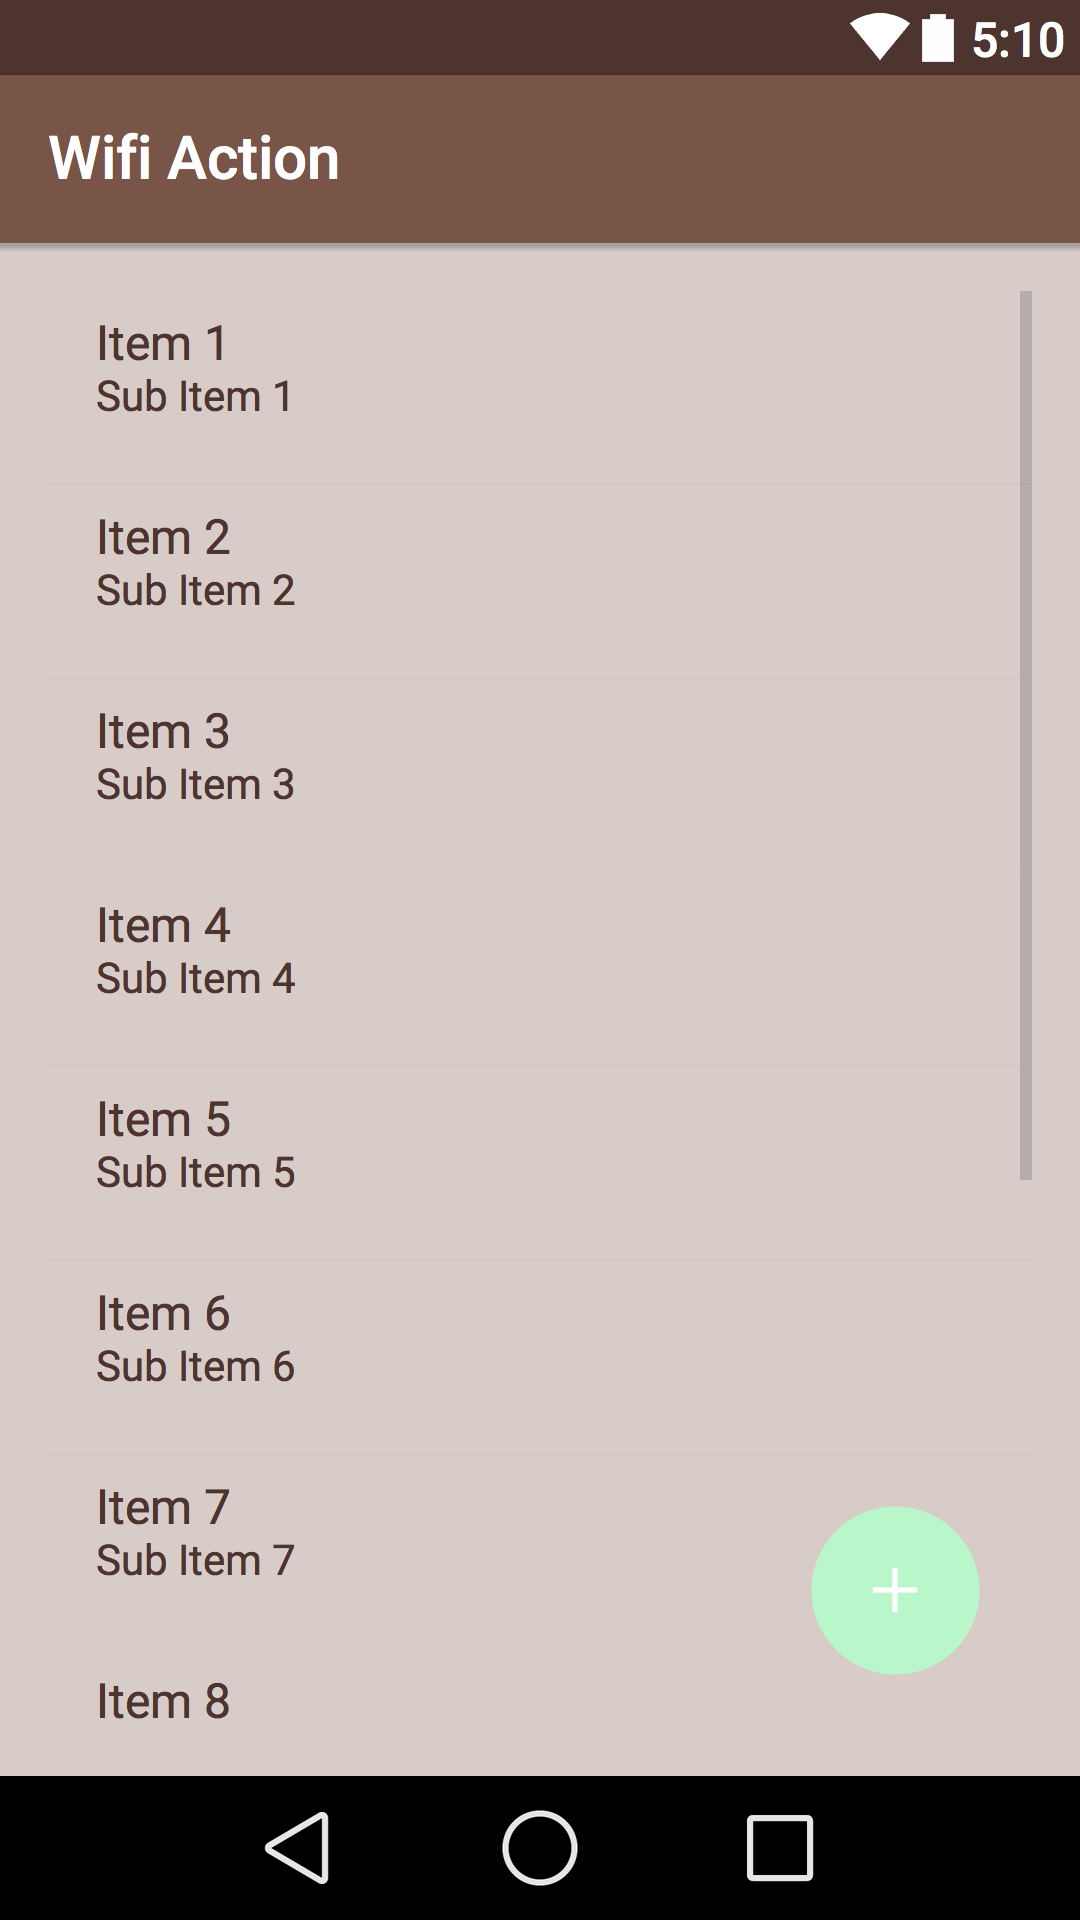
\includegraphics[width=0.4\textwidth]{images/mainactivity.png}
	\caption{Visuelle Repräsentation der MainActivity}
	\label{fig:mainactivity}
\end{figure}
Wenn die MainActivity gestartet wird, wird ein Asynchroner Job gestartet, welcher die serialisierten Aktion aus einer Datei lädt und anzeigt. Beim hinzufügen einer neuen Aktion werden alle Aktionen neu gespeichert damit keine verloren geht. Wenn eine Aktion in der Liste lange angeklickt wird, öffnet sich ein Kontext Menu, welches das löschen einer Aktion erlaubt. \\
Wird der Plus Button angeklickt werden alle bekannten Wireless LANs geladen und der ActionActivity übergeben. Das Laden der Wireless LANs ist mit Android einfach zu machen. \\
\begin{lstlisting}[language=Java]
	private ArrayList<Wifi> getKnownWifi() {
        WifiManager wifi = (WifiManager) getSystemService(Context.WIFI_SERVICE);
        List<WifiConfiguration> wifis = wifi.getConfiguredNetworks();
        ArrayList<Wifi> wifiList = new ArrayList<>();
        for(WifiConfiguration w : wifis) {
            wifiList.add(new Wifi(w.SSID,w.networkId););
        }
        return wifiList;
    }
\end{lstlisting}
Mit der Funktion getConfiguredNetworks() werden alle Wireless LANs ausgegeben mit denen das Mobiltelefon bereits eine Verbindung hatte.

\subsubsection{ActionActivity}
In der ActionActivity können neue Aktionen eingestellt und gespeichert werden. Im ersten Spinnerelement\footnote{In Android ist ein Spinnerelement eine Dropdown Liste} werden die Verfügbaren Aktionen angezeigt. Je nach Auswahl werden in der restlichen Ansicht unterschiedliche Felder angezeigt oder Versteckt. Deshalb überlagern sich gewisse Elemente in der Abbildung \ref{fig:actionctivity}. Im zweiten Spinnerelement werden die bekannten Wireless LANs angezeigt, welche von der MainActivity übergeben wurden. Die restlichen Elemente dienen der Einstellung der Aktion, welche über den Button \glqq Save\grqq{} gespeichert werden kann. Bei der Aktion Send SMS besteht die Möglichkeit eine Nummer aus dem Telefonbuch des Androidsystem auszuwählen. \\
\begin{lstlisting}[language=Java]
    public void onClick(View view) {
        Intent i = new Intent(Intent.ACTION_PICK, ContactsContract.CommonDataKinds.Phone.CONTENT_URI);
        startActivityForResult(i,REQUEST_CONTACTPICKER);
    }

    if(resultCode == RESULT_OK) {
        Uri contentUri = data.getData();
        Cursor cursor = getContentResolver().query(contentUri, null, null, null, null);
        cursor.moveToFirst();
        String number = cursor.getString(cursor.getColumnIndex(ContactsContract.CommonDataKinds.Phone.NUMBER));
        if(number.length() > 0) {
            etMessage3.setText(number);
        }
    }
\end{lstlisting}
Das Telefonbuch wird mit startActivityForResult gestartet und bei der Rückgabe wird der Eintrag aus dem Telefonbuch zurückgeben und ausgewertet. Dies hat den Vorteil dass die App nicht die Berechtigung zum lesen des Telefonbuches benötigt. Beim Drücken des \glqq Save\grqq{} Buttons werden die Daten zusammen gepackt und an die MainActivity zurück gegeben welche die Aktion speichert. \\
\begin{lstlisting}[language=Java]
-- ActionActivity.java -->
	Action a = new Action(etTitle.getText().toString(),((Wifi)spWifis.getSelectedItem()).getSsid(), at,cbOnConnect.isChecked(),cbOnLeave.isChecked());
	if(mActionType == 0) {
	    a.setStringParam1(etMessage3.getText().toString());
	} else {
	    a.setStringParam1(etMessage1.getText().toString());
	}
	a.setStringParam2(etMessage2.getText().toString());
	a.setBooleanParam1(swBoolean.isChecked());
	Intent i = new Intent();
	i.putExtra("ACTION",a);
	setResult(RESULT_OK, i);
	finish();
<----

-- MainActivity.java -->
	if(resultCode == RESULT_OK) {
		Action a = (Action) data.getSerializableExtra("ACTION");
		mActionList.add(a);
		actionAdapter.notifyDataSetChanged();
		saveActionList();
	}
<----
\end{lstlisting}
\begin{figure}[ht]
	\centering
	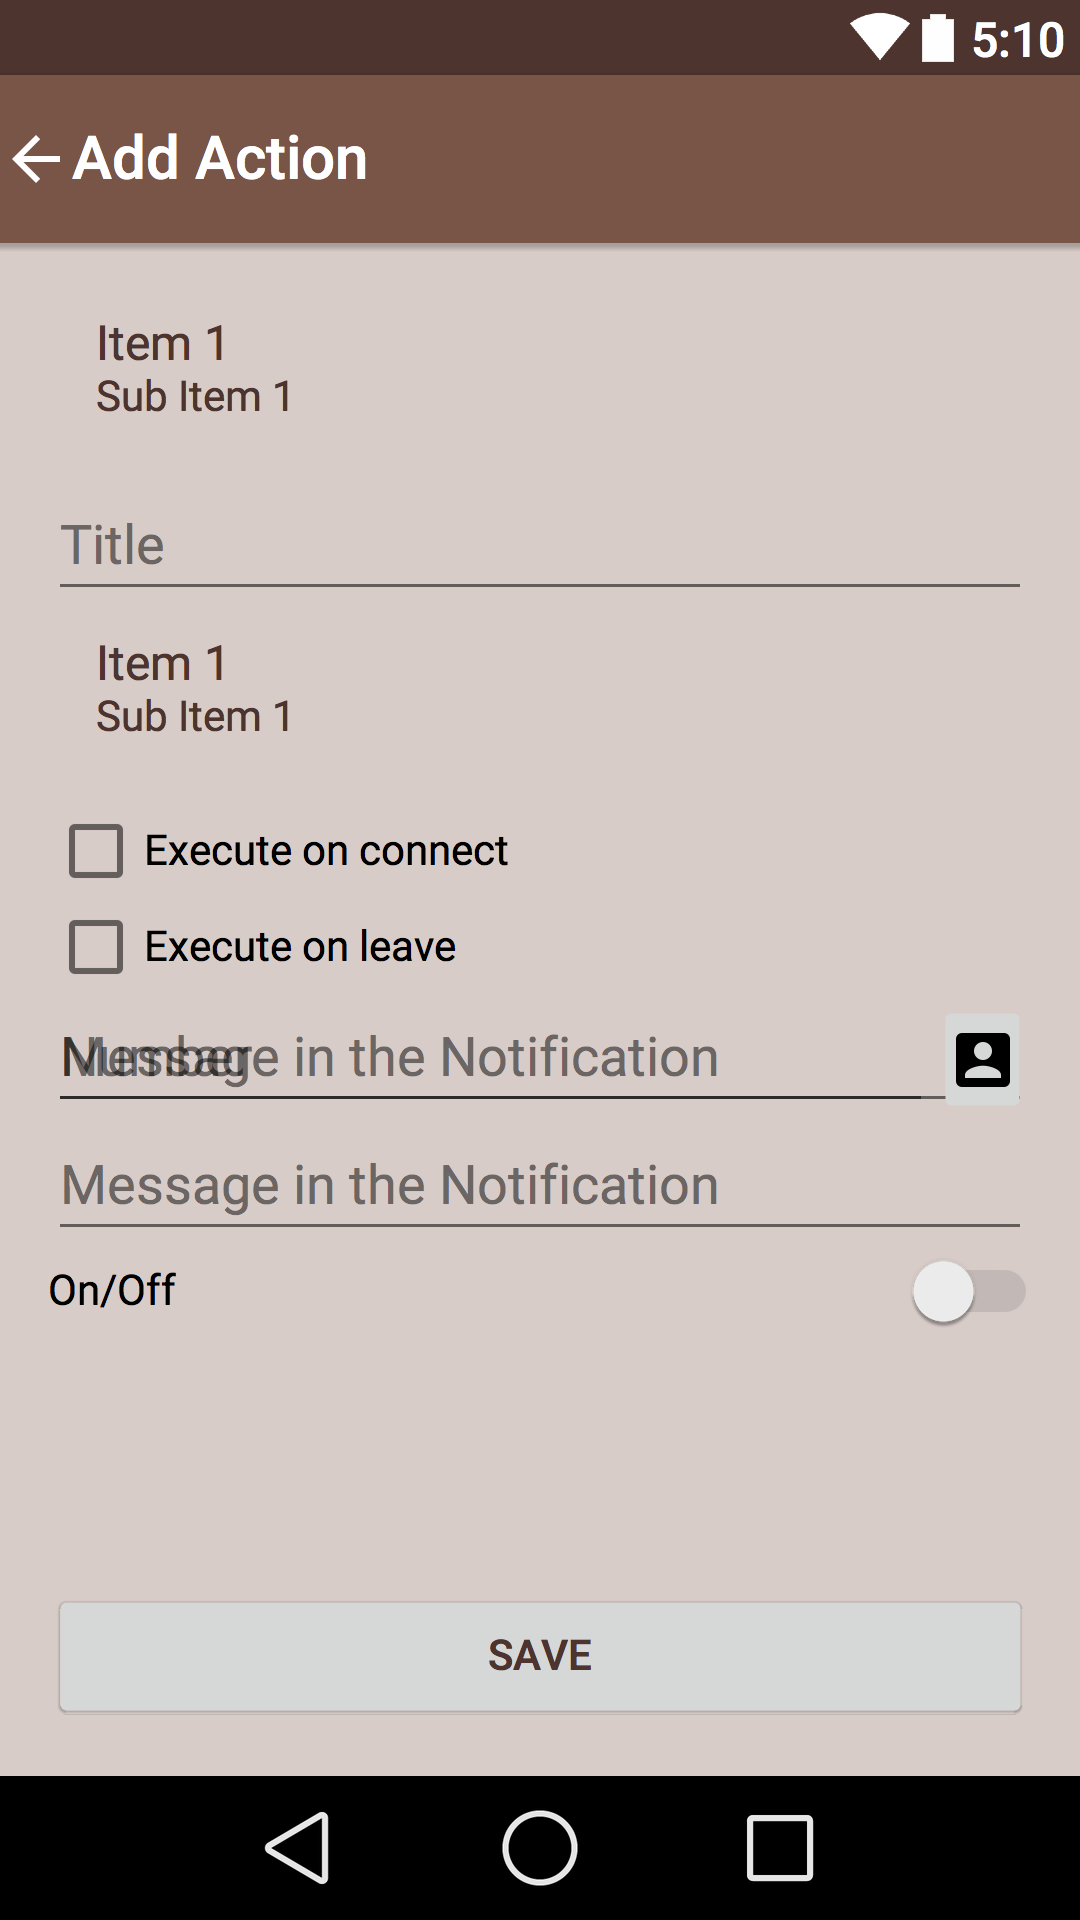
\includegraphics[width=0.4\textwidth]{images/actionactivity.png}
	\caption{Visuelle Repräsentation der ActionActivity}
	\label{fig:actionctivity}
\end{figure}

\subsubsection{LogActivity}
Die LogActivity ist im Vergleich zu den anderen Activities sehr schlicht. Aus einer Datenbank werden alle Log Einträge geladen und angezeigt. Der Adapter der ListView implementiert das ViewHolder Prinzip, welches auch bei sehr vielen Einträgen ein effizientes und für den Benutzer angenehmes Scrollen durch die Liste erlaubt.

% \begin{figure}[ht]
% 	\centering
% 	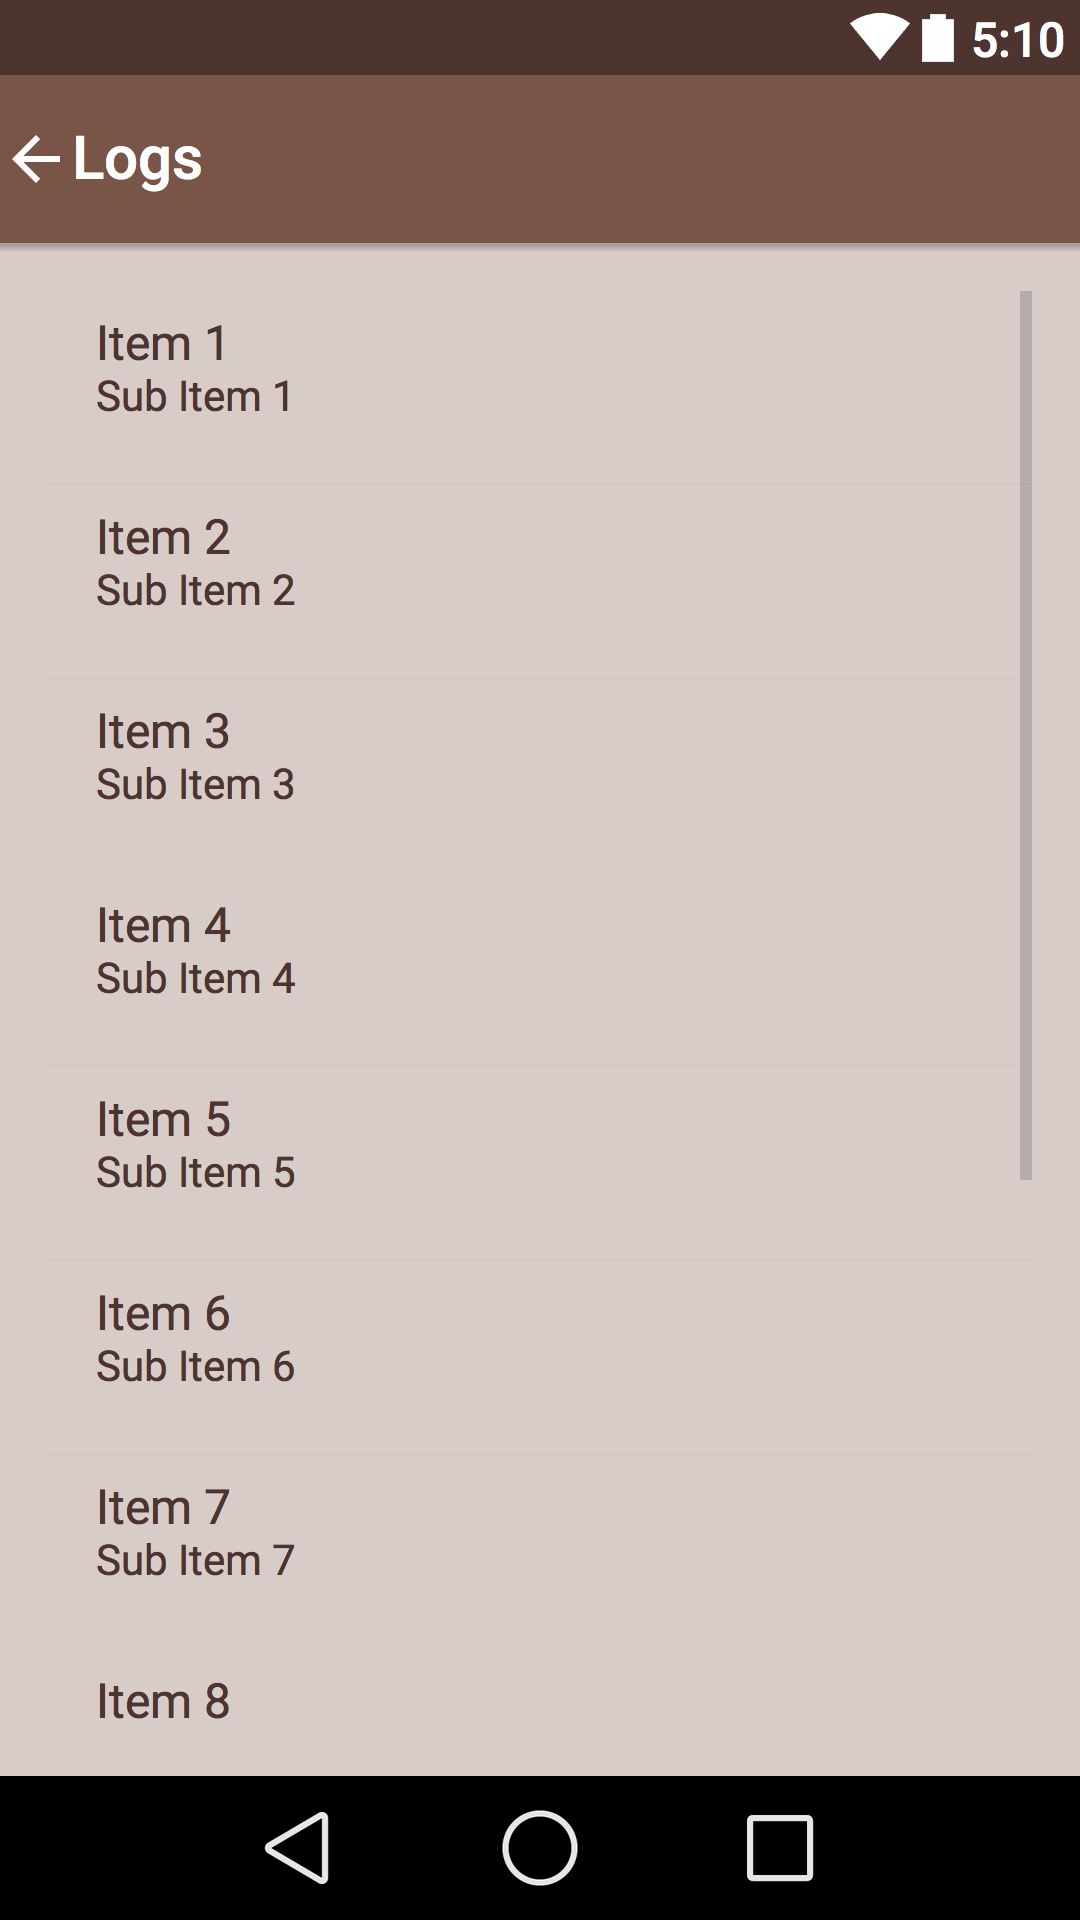
\includegraphics[width=0.4\textwidth]{images/logactivity.png}
% 	\caption{Visuelle Repräsentation der LogActivity}
% 	\label{fig:logactivity}
% \end{figure}

\newpage{}
\subsection{ConnectivityChangedReceiver}
Der ConnectivityChangedReceiver wird aktiviert und ausgeführt wenn es irgendeine Veränderung an der Netzwerkverbindung gibt. Diese Veränderung wird an den ActionService übergeben, welcher prüft ob eine Aktion ausgeführt werden muss. Dieser Ablauf ist im Sequenzdiagram in der Abbildung \ref{fig:seqactions} dargestellt.
\begin{figure}[ht]
    \centering
    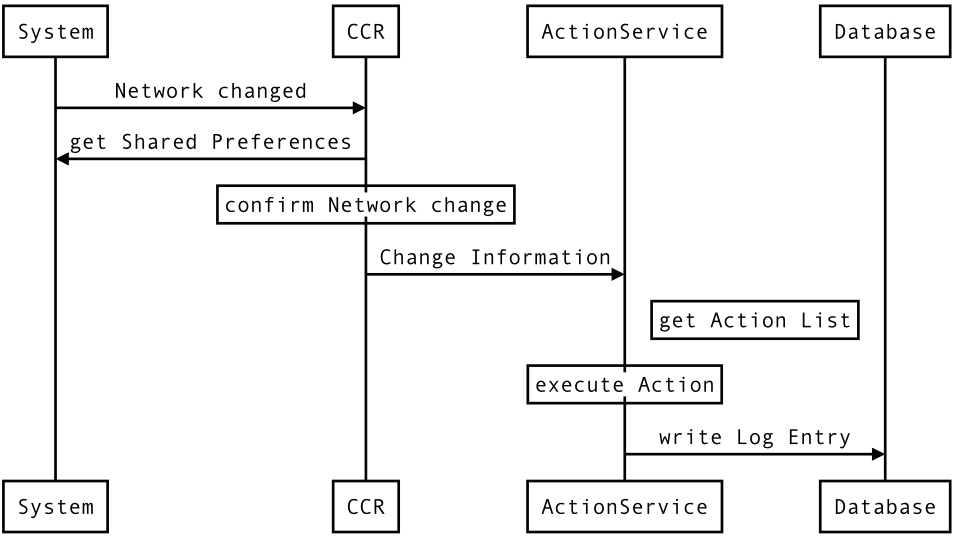
\includegraphics[width=0.8\textwidth]{images/seqActions.png}
    \caption{Sequenzdiagramm einer Netzwerkänderung}
    \label{fig:seqactions}
\end{figure}


 Der Receiver muss in der Lage sein zu wissen mit welchem Netzwerk das Mobiltelefon zuvor verbunden bzw. was der Status vor der Änderung der Netzwerkverbindung war. In einer ersten Implementation wurde dies mit Klassen Variabeln gelöst. Die Instanz des ConnectivityChangedReceiver lebt  aber nur während des Aufrufs und der Ausführung der onReceive Funktion. Darum ging der Wert der Variabeln nach kurzer Zeit Verloren. Die Lösung für dieses Problem heisst Shared Preferences. Mit den Shared Prefrences von Android können der Name und der Status der Netzwerkverbindung persistent gespeichert werden und bei der nächsten Ausführung von onReceive wieder gelesen werden. \\
\begin{lstlisting}[language=Java]
public void onReceive(Context context, Intent intent) {
    SharedPreferences sharedPreferences = context.getSharedPreferences("com.koki.app.wifiaction",Context.MODE_PRIVATE);
    String currentWifi = sharedPreferences.getString(CW,"");
    String currentState = sharedPreferences.getString(CS,"");
    ConnectivityManager cm = (ConnectivityManager) context.getSystemService(Context.CONNECTIVITY_SERVICE);
    NetworkInfo networkInfo = cm.getActiveNetworkInfo();
    if(networkInfo != null) {
        if(networkInfo.getTypeName().equals(currentState) && networkInfo.getExtraInfo().equals(currentWifi) ) {

        } else if (networkInfo.getTypeName().equals("WIFI") && !networkInfo.getExtraInfo().equals(currentWifi)) {
            ActionService.startAction(context, networkInfo.getExtraInfo(), true);
            sharedPreferences.edit().putString(CW, networkInfo.getExtraInfo()).putString(CS,networkInfo.getTypeName()).commit();
        } else if(currentState.equals("WIFI") && !networkInfo.getTypeName().equals("WIFI")) {
            ActionService.startAction(context, currentWifi, false);
            sharedPreferences.edit().putString(CW,networkInfo.getExtraInfo()).putString(CS,networkInfo.getTypeName()).commit();
        }
    }
}
\end{lstlisting}
In der Funktion onReceive wird überprüft ob der Verbindungstype gewechselt hat oder ob der Wireles LAN Netzwerkname geändert hat und die Funktion im ActionService mit den entsprechenden Parameter aufgerufen.

\subsection{ActionService}
Der ActionService erbt vom IntentService und wird beim Aufruf von onHandleIntent in einem eigenen Thread ausgeführt. Zuerst wird die Liste mit den Aktionen aus der Datei, welche die MainActivity schreibt, geladen. Danach wird überprüft ob für das aktuelle Wireless LAN und den Status der Verbindung eine Aktion existiert. Wird eine Aktion gefunden wird sie sogleich ausgeführt. Für jede Ausführung einer Aktion wird ein der Datenbank ein Log Eintrag erstellt. \\
\begin{lstlisting}[language=Java]
protected void onHandleIntent(Intent intent) {
    if (intent != null) {
        String wifi = intent.getStringExtra(EXTRA_WIFI);
        boolean isCon = intent.getBooleanExtra(EXTRA_ISCON,true);
        writeLog("WIFI CHANGE",wifi,isCon);
        ArrayList<Action> aList = loadFile();
        for(int i=0;i<aList.size();i++) {
            Action a = aList.get(i);
            if(a.getSsid().equals(wifi) && (a.isOnConnect() == isCon || a.isOnLeave() != isCon)) {
                switch(a.getActionType()) {
                    case BLUETOOTH:
                        handleActionBluetooth(a.isBooleanParam1());
                        break;
                    case GPS:
                        handleActionGPS(a.isBooleanParam1());
                        break;
                    case NOTIFICATION:
                        handleActionNotification(a.getStringParam1());
                        break;
                    case SMS:
                        handleActionSMS(a.getStringParam1(),a.getStringParam2());
                        break;
                }
                writeLog(a.getTitle(),wifi,isCon);
            }
        }
    }
}
\end{lstlisting}

\section{Restliche Implementationen}
Die Handhabung der Datenbank wurde mit einem neuen Framework namens Realm.io\footnote{Realm.io Mobile Database \url{http://realm.io/}} realisiert. Dieses Framework erleichtert das persistente Speichern sowie den Austausch von Daten zwischen verschiedenen Aktivitäten und Threads erheblich.